\documentclass[10pt,twocolumn]{article}
\usepackage[letterpaper,left=0.68in,right=0.68in,top=0.72in,bottom=0.72in,columnsep=0.20in]{geometry}
\usepackage[utf8]{inputenc}
\DeclareUnicodeCharacter{2212}{\ensuremath{-}}
\usepackage{graphicx,amsmath,amssymb,array,booktabs,url,hyperref}
\hypersetup{hidelinks}
\title{Auditing Flight-Phase Dependence in Unsupervised Aero-Engine Anomaly Detection: A Discovery-and-Confirmation Study on N-CMAPSS}
\author{Jinghang Mei\\School of Electrical and Computer Engineering\\The University of Sydney\\Sydney, Australia}
\date{}
\begin{document}
\maketitle
\begin{abstract}
Full-flight aero-engine anomaly scores may reflect normal operating-phase variation as well as health. Prior work has addressed changing operating conditions primarily through model adaptation and detection-performance improvements, while the stability of nominal healthy false-alarm calibration across flight phases has been less directly audited. Using N-CMAPSS, we treated DS02 as exploratory discovery data and evaluated residual PCA, Isolation Forest, and a causal LSTM sequence-reconstruction network. We examined operating-condition correction sensitivity, phase-wise healthy row-level false-positive rates (FPRs), and cross-phase threshold transfer before applying a frozen protocol once to the DS03 independent confirmatory subset. At the primary nominal 1\% pooled calibration target, DS02 climb/cruise/descent FPRs were 0.125\%/0.428\%/3.459\% for PCA, 0.268\%/0.558\%/2.487\% for the Isolation Forest seed mean, and 0.488\%/0.729\%/2.080\% for the LSTM seed mean. In exploratory DS02 PCA sensitivity analysis, the tested static, derivative-based, and finite-history correction schemes did not eliminate the observed dependence. On DS03, the corresponding FPRs were 0.877\%/0.912\%/1.977\%, 0.409\%/1.104\%/2.142\%, and 0.751\%/1.889\%/2.215\%; the pre-specified pooled directional pattern was reproduced. Engine- and seed-level heterogeneity remained, and some LSTM descent-minus-cruise bootstrap intervals included zero. These results motivate explicit phase-stability auditing alongside aggregate anomaly-detection evaluation under nonstationary operating conditions.
\end{abstract}
\par\smallskip\noindent\textbf{Keywords---} 
Aero-engine anomaly detection; N-CMAPSS; false-alarm calibration; flight phases; threshold transfer.


\section{Introduction}\label{introduction}

Aero-engine health monitoring must identify developing faults early while keeping false alarms manageable. A threshold that detects weak changes but repeatedly alarms during healthy operation can impose unnecessary review and reduce the usefulness of the warning stream. False-alarm probability has therefore long been an explicit design consideration in engine anomaly detection and alert-threshold placement {[}2{]}, {[}11{]}. The present study concerns the healthy-alarm side of that trade-off; it does not evaluate fault-detection sensitivity or operational response.

The detectors are unsupervised with respect to fault labels; supplied health-state annotations are used only to select healthy samples for retrospective fitting, calibration, and evaluation.

Full-flight monitoring complicates the interpretation of a sensor departure. A measured vector may be viewed schematically as \(x_t=f(h_t,o_t,d_t,\epsilon_t)\), where \(h_t\) denotes engine health, \(o_t\) the operating point, \(d_t\) normal operating dynamics, and \(\epsilon_t\) measurement and model error. This expression is conceptual, not an identified causal model. Earlier C-MAPSS studies often used restricted operating snapshots, whereas N-CMAPSS simulates complete flights driven by recorded flight conditions, including climb, cruise, and descent {[}1{]}. Variation with operating context may therefore alter healthy anomaly scores even when health state is unchanged. {[}2{]}, {[}10{]}.

An aggregate calibration target does not itself guarantee stable conditional performance. In particular, \(P(\mathrm{alarm}\mid\mathrm{healthy})\) is an exposure-weighted mixture of \(P(\mathrm{alarm}\mid\mathrm{healthy},\mathrm{phase})\) over the phases represented in the calibration set. The aggregate may satisfy its nominal target while climb, cruise, and descent have materially different healthy false-positive rates. Healthy false-positive rate (FPR) is interpreted here as the healthy false-alarm rate. Thresholds learned in one healthy phase may likewise transfer unevenly to another. The phase labels in this study are retrospective full-flight strata, not outputs of an online phase detector.

Flight-condition-aware monitoring, normalization, regime-specific models, and adaptive thresholds are established prior art {[}3{]}, {[}4{]}, {[}6{]}AS.1943-5525.0001483). N-CMAPSS has also been used for anomaly detection and for increasingly sophisticated temporal modelling {[}7{]}, {[}8{]}, {[}9{]}. The question here is narrower than improving a detector: whether nominal pooled healthy FPR calibration remains stable across normal flight phases under full-flight operation.

The DS02 discovery dataset supplied exploratory development, including correction-specification robustness and cross-detector checks. The detector, correction, phase, calibration, endpoint, and directional interpretation rules were then frozen before a one-shot evaluation on the DS03 independent confirmatory subset. The DS03 official-test arrays were not used for method development. The study consequently makes no claim about fault sensitivity or real-aircraft deployment.

The study addresses three research questions: RQ1, do healthy anomaly scores and healthy row-level FPRs vary systematically across flight phases? RQ2, do the tested static, derivative-based, and finite-history operating-condition corrections eliminate the observed dependence? RQ3, does the pooled directional pattern reproduce across three tested detector implementations and a frozen confirmatory N-CMAPSS subset?

The contributions are:

\begin{enumerate}
\def\labelenumi{\arabic{enumi}.}
\tightlist
\item
  A controlled audit of phase-dependent healthy false-alarm calibration under full-flight N-CMAPSS operation, including cross-phase threshold transfer.
\item
  An exploratory PCA correction challenge in which the tested static, derivative-based, and finite-history schemes did not eliminate the observed DS02 dependence; separately, the pattern was observed across three tested detector implementations under the common history correction.
\item
  A discovery-and-confirmation design in which the protocol developed on DS02 was frozen before a one-shot directional evaluation on previously unseen DS03 official-test data.
\end{enumerate}

These contributions concern calibration-stability evidence in the specified simulated N-CMAPSS subsets, not a new detector, a causal explanation, or deployment validation.

\section{Related Work}\label{related-work}

\subsection{Operating Context in Full-Flight Monitoring}\label{operating-context-in-full-flight-monitoring}

Classical aero-engine monitoring often used a restricted operating point or corrected measurements to a reference condition. The original N-CMAPSS data descriptor contrasts the earlier snapshot-oriented C-MAPSS benchmark with simulated complete flights driven by recorded flight profiles {[}1{]}. Flight-condition-aware monitoring predates N-CMAPSS: flight-stage normalization of health and usage monitoring indicators was described by Noura and Wiig {[}4{]}, and flight-data interrelations were modelled within a specified flight regime by earlier engine-health work {[}3{]}. Fleet-monitoring studies have also combined adaptive engine-performance models with probabilistic diagnosis across variable conditions {[}5{]}. Regime-specific modelling and operating-condition normalization are therefore not methodological novelties of the present study. A recent N-CMAPSS cruise-stage RUL benchmark makes the complementary choice to restrict analysis to a more stable flight stage for model comparability {[}10{]}; the present audit retains all three retrospectively defined phases to examine calibration transfer.

\subsection{Detection Modelling Versus Calibration Stability}\label{detection-modelling-versus-calibration-stability}

Reconstruction and one-class approaches have long supplied anomaly scores for monitoring. Ulmer \emph{et al.} used N-CMAPSS DS02 to study training-data contamination and unsupervised refinement with residual-based models, emphasizing anomaly-detection performance rather than phase-conditional healthy calibration {[}7{]}. Ramírez \emph{et al.} evaluated information-based fault detection on N-CMAPSS {[}8{]}. More recent N-CMAPSS work evaluates a physics-guided spatiotemporal graph model primarily through detection metrics such as ROC-AUC and F1 {[}9{]}. These studies establish that N-CMAPSS anomaly detection, temporal architectures, and cross-model performance comparisons are not new. They do not make an unchanged pooled healthy threshold's climb/cruise/descent FPR and cross-phase transfer the central endpoint, as done here.

\subsection{False-Alarm Decisions and Operational Burden}\label{false-alarm-decisions-and-operational-burden}

False-alarm-aware evaluation and context-specific thresholds are also established. Borguet \emph{et al.} derived an engine anomaly threshold from a specified false-alarm probability and assessed detection decisions and delay {[}2{]}. Massé \emph{et al.} examined alert-threshold placement and repeated threshold crossings for aircraft-engine abnormality scores {[}11{]}. Zhao \emph{et al.} proposed adaptive aero-engine thresholds across flight-envelope subareas {[}6{]}AS.1943-5525.0001483). These precedents show why an aggregate ROC-AUC or F1 score cannot by itself characterize the healthy-alarm workload at a selected operating threshold. Repeated false alarms may also have a ``cry-wolf'' consequence in warning systems, although that human response is not measured in the present N-CMAPSS study {[}12{]}00060-7). Flight-level alarm burden is consequently reported only as a secondary, exposure-dependent descriptive endpoint, not as evidence of operator behavior.

Existing aero-engine monitoring studies address operating-condition variability through regime-specific models, normalization, adaptive thresholds, and increasingly sophisticated temporal architectures. However, the representative work above does not make phase stability of a nominal pooled healthy-FPR calibration its primary held-out evaluation target. This is the narrow gap addressed here; no claim is made to priority in phase-aware monitoring or adaptive thresholding.

\section{Methodology}\label{methodology}

\subsection{Dataset and Discovery--Confirmation Design}\label{dataset-and-discoveryconfirmation-design}

The analysis used the N-CMAPSS DS02 discovery dataset for exploratory development and the DS03 independent confirmatory subset for frozen confirmation. DS02 supported examination of operating-condition correction, phase-stratified false alarms, and sensitivity analyses. The detector families, correction specification, calibration rule, phase definition, evaluation endpoints, and interpretation rule were fixed before the DS03 official-test outcomes were examined. DS03 was evaluated once under the frozen primary protocol; DS02 estimates were not treated as independent confirmation.

Engine was the partitioning and top-level inferential unit; timestamped observations were nested within flights identified by engine and cycle. The available data retained the official development and test divisions. Only measured sensor channels and operating descriptors entered the anomaly-scoring pipeline. Dataset labels, engine and flight identifiers, health-state labels, and derived phase labels served partitioning, sequence grouping, or evaluation roles, not numerical detector features.

\subsection{Data Partitioning and Leakage Controls}\label{data-partitioning-and-leakage-controls}

For DS02, model-fitting engines were 2, 5, 10, and 16; threshold-calibration engines were 18 and 20; and official-test engines were 11, 14, and 15. LSTM epoch selection used engines 2, 5, and 10 for fitting and engine 16 for validation. After epoch selection, the correction and network were refitted using all DS02 model-fitting engines; neither calibration nor official-test engines contributed to epoch selection.

For DS03, the frozen development-engine allocation assigned engines 1, 2, 3, 5, 6, 7, and 9 to model fitting and engines 4 and 8 to threshold calibration. The official-test audit comprised engines 10 through 15. Within the fit set, engines 1, 2, 3, 5, 6, and 7 were used for LSTM epoch-selection fitting and engine 9 for validation. The operating regression, residual scaling, and detector parameters were fitted without calibration or official-test data. Calibration thresholds were locked before the DS03 official-test arrays were opened. No detector, correction, or threshold setting was changed after audit outcomes were available.

\subsection{Healthy-State and Flight-Phase Definitions}\label{healthy-state-and-flight-phase-definitions}
\begin{figure*}[t]
\centering
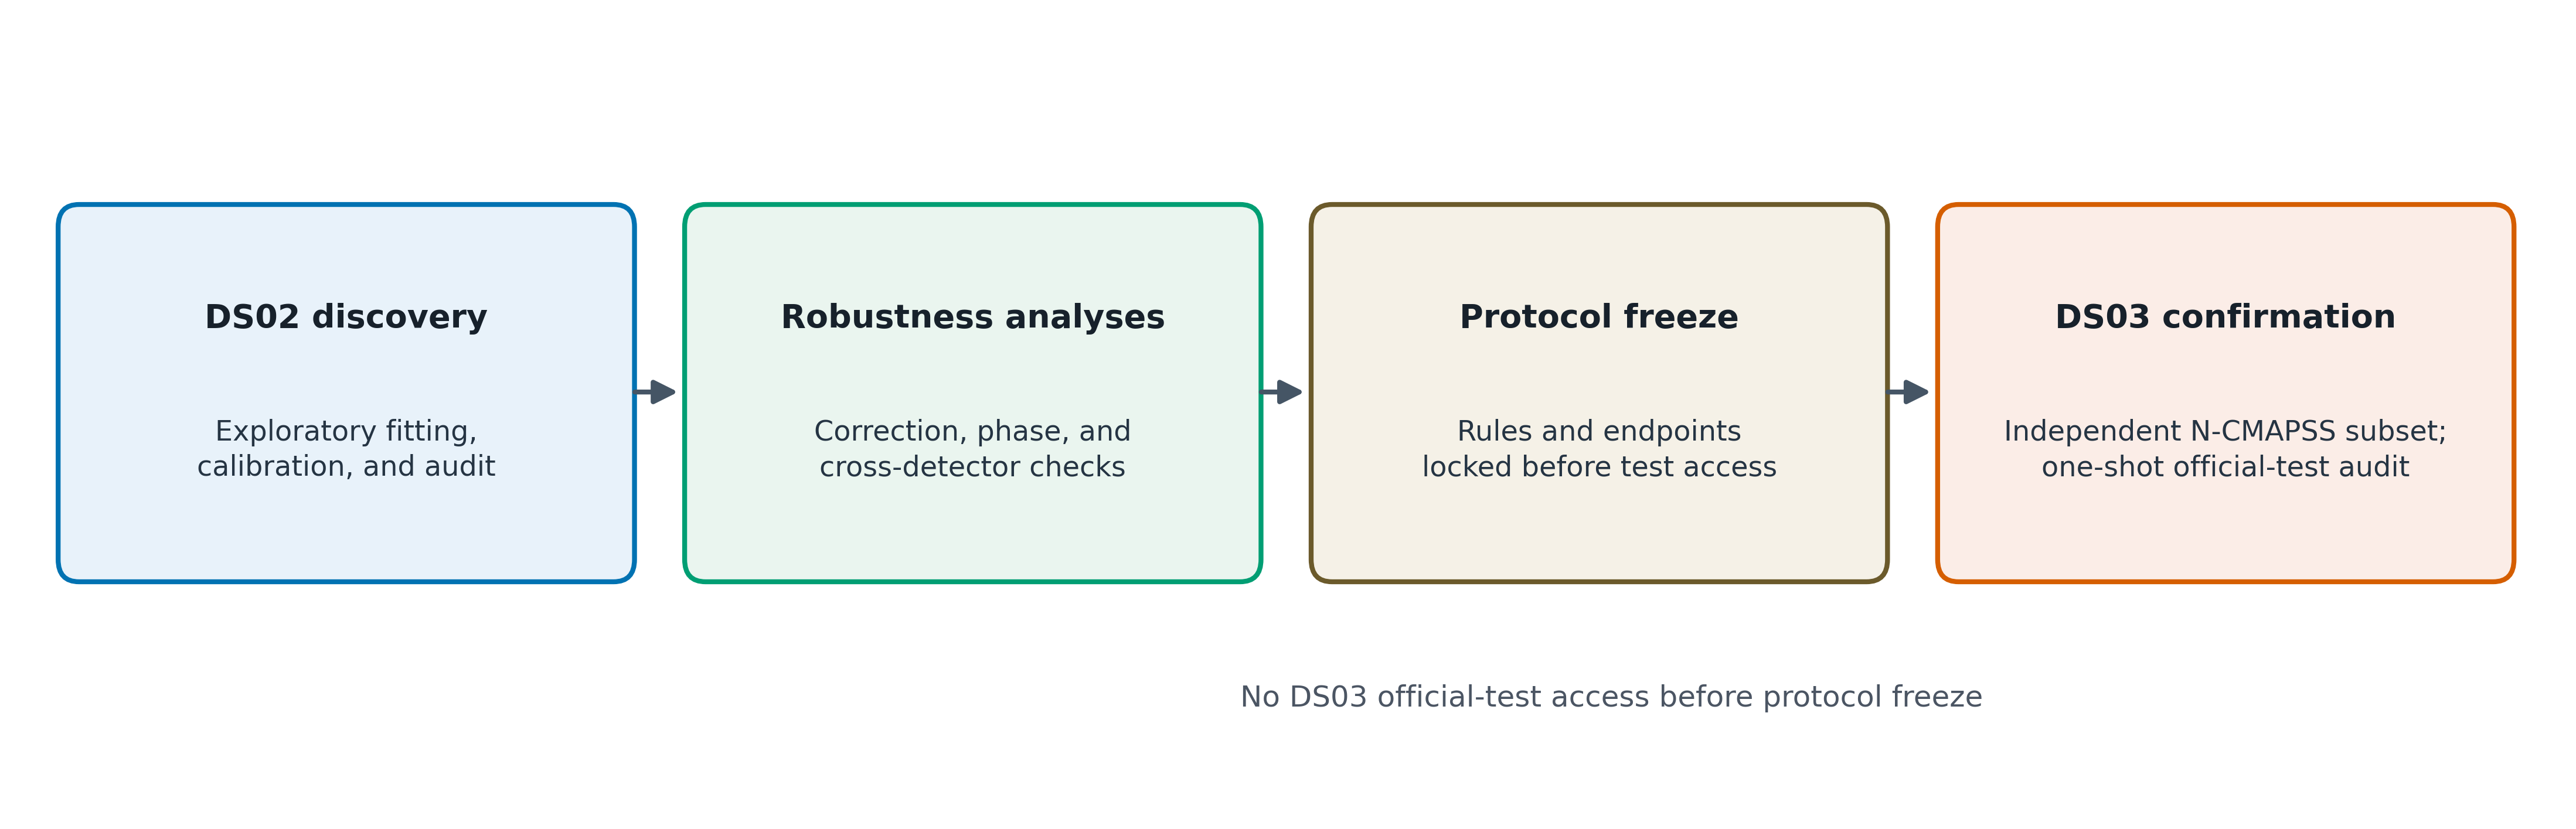
\includegraphics[width=0.94\textwidth]{figures/figure_1_study_design.png}
\caption{Discovery-to-confirmation study design. DS02 discovery and exploratory robustness analyses preceded protocol freeze; DS03 is an independent confirmatory subset evaluated once after freeze. No DS03 official-test access occurred before freeze.}
\end{figure*}

The detectors used 14 measured sensor channels as their anomaly-detection variables. Altitude, Mach number, throttle-resolver angle, and inlet temperature were operating descriptors for residualization; they were not health-state or phase labels. The health-state field imposed an oracle healthy-row restriction on fitting, threshold calibration, and retrospective healthy false-alarm evaluation. It was never passed as a detector feature. Accordingly, the reported false-alarm endpoints do not measure detection of faulty-state observations.

For each complete flight, the primary cruise interval ran from the first through the last sample whose altitude reached at least 90\% of that flight's observed altitude range above its minimum. Earlier samples were labeled climb and later samples descent. These labels require the complete flight trajectory and were used only for retrospective stratification and phase-specific auditing; the procedure is not an online phase detector. An alternative altitude-rate phase rule was examined within DS02 discovery but was not part of the frozen DS03 confirmation.

\subsection{Operating-Condition Correction}\label{operating-condition-correction}

The exploratory DS02 correction comparison considered a static operating-state basis, a static-plus-first-difference basis, and a finite-history basis. The final-validation and frozen-confirmation detector analyses used the history specification. For each flight, the history descriptors comprised current operating state, first differences, and trailing means, standard deviations, and endpoint slopes over 30- and 120-sample windows, corresponding to 30 and 120 s at the dataset's 1-Hz sample rate. Descriptor construction reset at flight boundaries and did not use future samples.

A ridge-regularized regression predicted measured sensors from the operating descriptors. The basis included cubic terms of the instantaneous operating state, linear and squared dynamic terms, and interactions between instantaneous state and its first differences. The frozen ridge penalty was 1.0. Regression fitting and residual standardization used model-fitting engines only. The same fitted transformation was applied to the disjoint calibration and audit engines. The static/derivative/history comparison remained exploratory; the history correction was carried forward without using DS03 outcomes to choose among variants.

\subsection{Detector Implementations}\label{detector-implementations}

PCA was fitted to standardized operating-regression residuals with five components and full singular-value decomposition. Its row score was mean squared residual reconstruction error. Isolation Forest used 200 trees, a maximum sample size of 8192 per tree, and automatic contamination; negative \texttt{score\_samples} was used so larger scores indicated greater anomaly. Stochastic detectors were run with seeds 0, 1, and 2.

The LSTM detector was a causal LSTM sequence-reconstruction network. Within each flight, training formed nonoverlapping 256-row windows; incomplete training windows were omitted. A forward LSTM with 16 hidden units produced a hidden state at each time step. A tanh-activated dense layer mapped each state to eight features, a second forward LSTM with 16 hidden units processed that per-time-step representation, and a final dense layer reconstructed the sensor-residual vector at each time step. Thus the eight-feature layer was a time-step bottleneck, not a single sequence-level latent code. At scoring, incomplete final windows were zero-padded, and each observed row received its own mean squared feature-reconstruction error. The forward recurrence used current and preceding samples within a window, not future samples.

Network fitting used Adam with learning rate 0.001 and batches of 256 sequences. Epoch selection used engine-disjoint validation with a maximum of 600 epochs, patience of six epochs, and a minimum monitored improvement of 0.0001; the selected epoch count was then used for a fresh fit on all model-fitting engines. The DS02 seed-0 selection reached the epoch ceiling and was retained as a convergence limitation, without test-informed retuning.

\subsection{Calibration and Statistical Analysis}\label{calibration-and-statistical-analysis}

For each detector and seed, pooled healthy calibration scores set nominal pooled healthy row-level FPR targets of 0.5\%, 1\%, and 2\% by the empirical upper quantile with the \texttt{higher} order-statistic rule. The 1\% target was primary. A healthy audit row was alarmed only when its score exceeded the locked threshold. Overall and phase-specific healthy row-level FPRs were calculated as alarmed healthy rows divided by eligible healthy rows, pooled and separately by engine. Directional contrasts were descent minus climb and descent minus cruise. For cross-phase transfer, a threshold was calibrated within one phase and applied to each audit phase; the summary endpoint was the maximum off-diagonal false-positive rate. Flight-level burden was summarized separately as the fraction of healthy flights with any alarm and the mean number of contiguous alarm events per healthy flight.

Uncertainty for the primary pooled endpoints used 2000 hierarchical bootstrap replicates and percentile 95\% confidence limits. Calibration and audit data were resampled separately: engines were sampled with replacement, then flights were sampled with replacement within each selected engine. Each replicate re-estimated the pooled and phase-specific calibration thresholds and recomputed the audit rates, contrasts, and maximum off-diagonal transfer rate. Timestamps were not treated as independent inferential units, and timestamp-level significance tests were not used. Intervals pertain to individual detector runs; no interval for an arithmetic mean across stochastic seeds was executed. The frozen DS03 directional rule assessed the signs of the pooled PCA contrasts and the pooled seed-mean contrasts for each stochastic detector, with per-engine exceptions reported separately.

\section{Results}\label{results}

\subsection{Discovery of Phase-Dependent Healthy False Alarms on DS02}\label{discovery-of-phase-dependent-healthy-false-alarms-on-ds02}

At the primary nominal 1\% pooled calibration target, PCA healthy row-level FPR was 0.125\% in climb, 0.428\% in cruise, and 3.459\% in descent. The descent-minus-climb and descent-minus-cruise contrasts were +3.335 and +3.031 percentage points (pp), respectively.

The corresponding Isolation Forest seed-mean FPRs were 0.268\%, 0.558\%, and 2.487\%, with contrasts of +2.219 and +1.928 pp.~For the causal LSTM sequence-reconstruction network, the seed-mean FPRs were 0.488\%, 0.729\%, and 2.080\%, with contrasts of +1.592 and +1.351 pp.~Descent therefore had the highest pooled healthy FPR across the three tested implementations. The nominal 1\% target applied to pooled healthy calibration scores; it did not constrain each audit phase to 1\% FPR or imply uniform direction in every engine.

\subsection{Sensitivity to Operating-Condition Correction}\label{sensitivity-to-operating-condition-correction}

In the executed DS02 exploratory PCA comparison, the static correction yielded climb, cruise, and descent FPRs of 0.146\%, 0.583\%, and 3.001\%. The static-plus-derivative correction yielded 0.061\%, 0.457\%, and 3.106\%, whereas finite-history correction yielded 0.125\%, 0.428\%, and 3.459\%. All values used the primary phase rule and nominal 1\% calibration target.

Descent-minus-climb contrasts were +2.854, +3.045, and +3.335 pp for static, static-plus-derivative, and finite-history correction, respectively; descent-minus-cruise contrasts were +2.418, +2.648, and +3.031 pp in the same order. In DS02 exploratory PCA analysis, static, derivative-based, and finite-history corrections did not eliminate the phase-dependent FPR pattern. This correction comparison was not independently repeated on DS03. Cross-detector consistency was evaluated under the selected finite-history correction.

\subsection{Consistency Across Three Detector Implementations}\label{consistency-across-three-detector-implementations}

With the common history correction and pooled calibration, DS02 overall healthy row-level FPRs were 1.363\% for PCA, 1.127\% for the Isolation Forest seed mean, and 1.118\% for the LSTM seed mean. The descent elevation was observed across three tested detector implementations under a shared preprocessing and calibration protocol. The comparison is limited to those implementations.

The Isolation Forest descent-minus-climb contrast spanned +2.050 to +2.416 pp across the tested seeds; the LSTM contrast spanned +1.521 to +1.628 pp.~These ranges describe all tested seeds, not uncertainty intervals for their means. Final LSTM validation superseded the earlier short-run baseline. The DS02 LSTM seed-0 run reached the pre-specified 600-epoch ceiling while its validation loss was still improving over the final monitored windows; it was not classified as converged.

\subsection{Cross-Phase Threshold Transfer}\label{cross-phase-threshold-transfer}

On DS02, the worst off-diagonal healthy row-level FPR after phase-specific calibration was 15.555\% for PCA; the arithmetic means of the per-seed maxima were 27.281\% for Isolation Forest and 5.954\% for LSTM. The corresponding DS03 values were 6.716\%, 9.386\%, and 5.308\%. Each per-run maximum is over cross-phase transfer cells, not a phase FPR obtained with the pooled calibration threshold. The transfer values show that phase-calibrated thresholds did not perform uniformly across healthy phases.

For every evaluated detector/seed run on both subsets, the maximum off-diagonal cell applied a threshold calibrated on healthy climb rows to healthy descent rows. Thus, the calibration phase was climb and the audit phase was descent for the reported maxima. The stochastic-detector aggregate values above are means of the per-seed maxima, not maxima computed after averaging seed-specific transfer matrices.

\subsection{Cluster-Aware Uncertainty and Heterogeneity}\label{cluster-aware-uncertainty-and-heterogeneity}
\begin{figure*}[t]
\centering
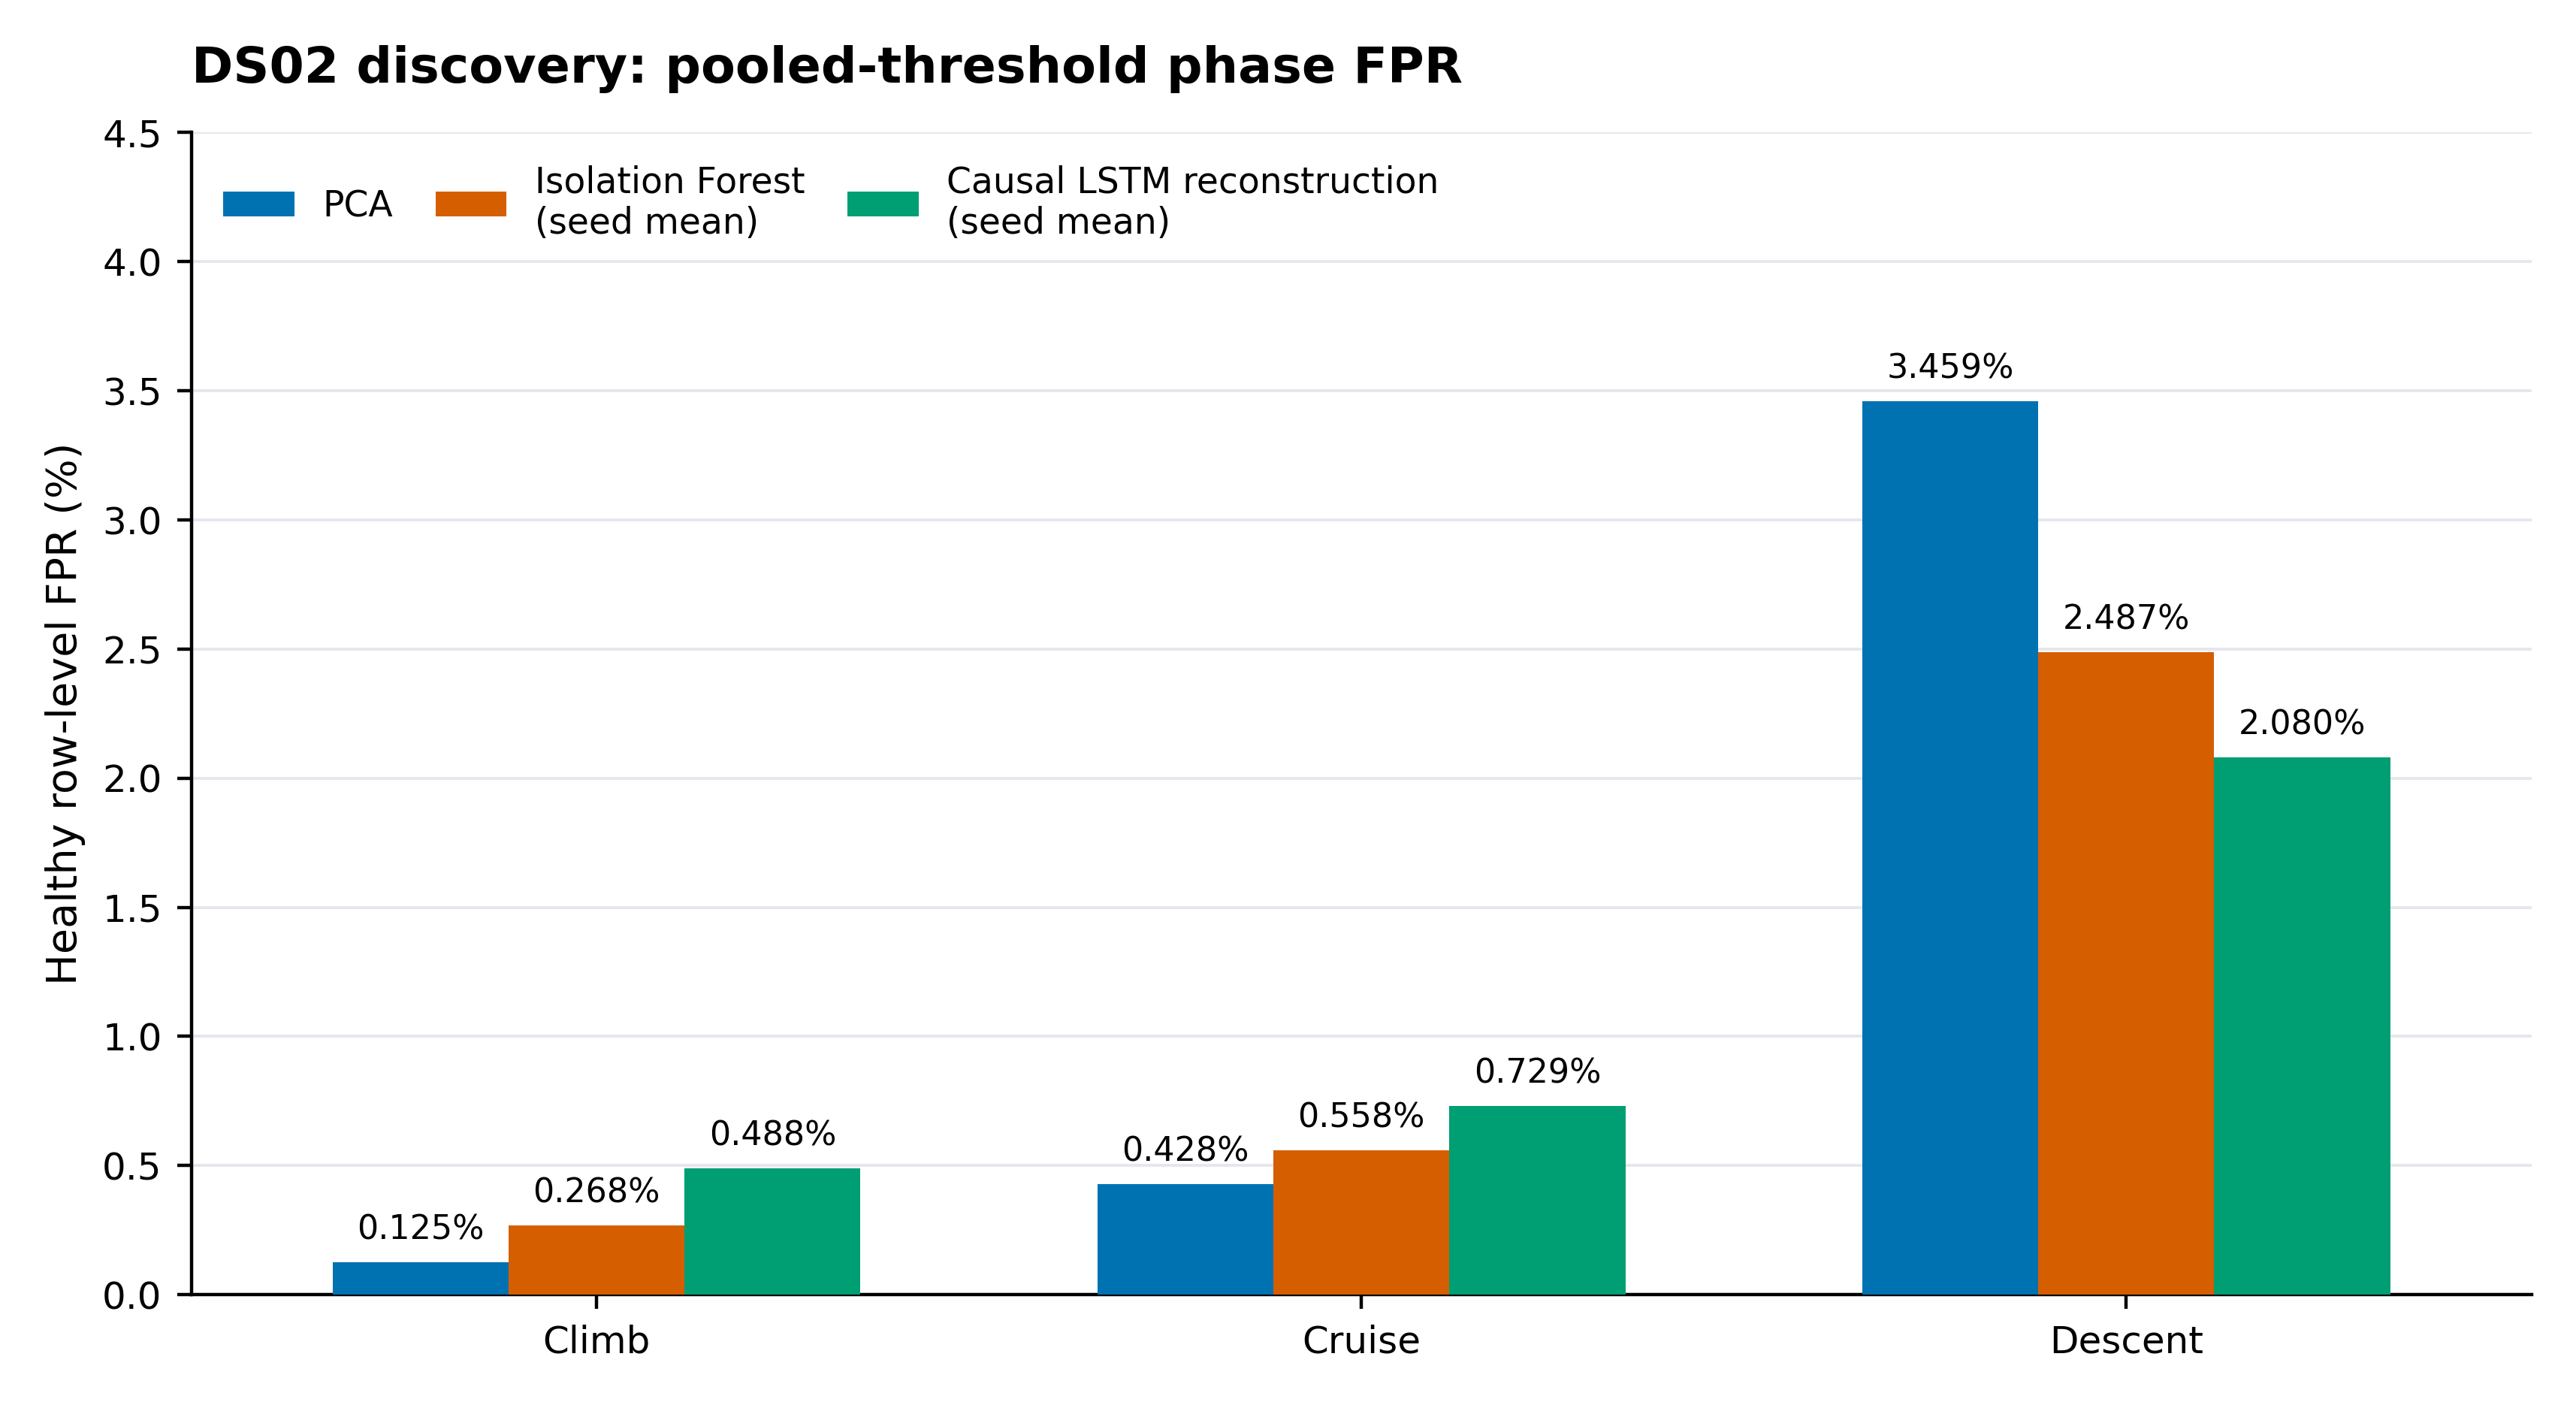
\includegraphics[width=0.94\textwidth]{figures/figure_2_ds02_phase_fpr.png}
\caption{DS02 exploratory healthy row-level FPR at the nominal 1\% pooled calibration target. PCA is a single run; Isolation Forest and the causal LSTM sequence-reconstruction network are arithmetic three-seed means. Bars show pooled-threshold phase FPR, not cross-phase transfer FPR. Figures 2 and 4 use the same vertical scale to support direct visual comparison.}
\end{figure*}

The official healthy audit sets contain only three DS02 engines and six DS03 engines. Individual-engine reversals therefore represent a material fraction of the available generalization units and should not be interpreted as negligible edge cases.

For DS02 PCA, hierarchical-bootstrap 95\% intervals were {[}+2.070, +5.629{]} pp for descent-minus-climb and {[}+1.808, +5.261{]} pp for descent-minus-cruise. All tested Isolation Forest seeds had positive intervals for both contrasts. By contrast, the DS02 LSTM descent-minus-climb intervals for seeds 1 and 2 included zero: {[}−0.022, +2.817{]} and {[}−0.347, +2.802{]} pp.~At the engine level, DS02 engine 14 had negative LSTM descent-minus-climb contrasts for seeds 1 and 2 (−0.158 and −0.521 pp), despite the positive pooled seed-mean contrast. These two reversals occur within an audit set of only three engines.

On DS03, the PCA intervals were {[}+0.434, +1.785{]} pp for descent-minus-climb and {[}+0.560, +1.573{]} pp for descent-minus-cruise. Each Isolation Forest seed had a positive interval for both contrasts. The LSTM descent-minus-climb intervals were positive for all seeds, but every LSTM descent-minus-cruise interval included zero. The engine-then-flight bootstrap accounts for clustering and recalibrates thresholds within replicates; with limited engines, these intervals summarize uncertainty for the observed N-CMAPSS engine sets rather than precise population-level effects. These are individual-seed intervals, not intervals for the fixed three-seed arithmetic mean. No timestamp-level p-values were used.

\subsection{Frozen DS03 Confirmation}\label{frozen-ds03-confirmation}

DS02 served as the exploratory discovery dataset. DS03 came from the official NASA distribution and was evaluated as an independent confirmatory subset after the protocol was frozen. Its development data supported model fitting and threshold calibration under that protocol; official-test arrays were opened once, after fitting and calibration were locked. At the pre-specified primary target, pooled PCA climb, cruise, and descent FPRs were 0.877\%, 0.912\%, and 1.977\%; the corresponding Isolation Forest seed means were 0.409\%, 1.104\%, and 2.142\%; and LSTM seed means were 0.751\%, 1.889\%, and 2.215\%.

The pooled descent-minus-climb and descent-minus-cruise contrasts were +1.100 and +1.066 pp for PCA, +1.733 and +1.038 pp for the Isolation Forest seed mean, and +1.464 and +0.325 pp for the LSTM seed mean. Thus, the pre-specified pooled directional pattern was reproduced. Stochastic-detector seed means are descriptive point summaries rather than inferential estimates; no seed-mean confidence intervals are available.

Three of 42 per-engine detector/seed rows were directional exceptions within only six official-test engines, all for LSTM seed 2: engine 12 had a descent-minus-climb contrast of −0.086 pp, and engines 13 and 15 had descent-minus-cruise contrasts of −0.105 and −0.034 pp.~In addition, all three individual-seed DS03 LSTM descent-minus-cruise 95\% intervals included zero: {[}−0.222, +1.201{]}, {[}−0.270, +1.158{]}, and {[}−0.582, +1.025{]} pp for seeds 0, 1, and 2, respectively. The pooled pattern therefore reproduced without uniform engine-level replication or a positive interval for every individual LSTM contrast.

\subsection{Exploratory DS02 Phase-Rule Sensitivity}\label{exploratory-ds02-phase-rule-sensitivity}

The alternative retrospective rule identified cruise between the first and last points meeting at least 85\% of each flight's altitude range and an absolute centered 60-second altitude rate of at most 2 altitude units per second. At the nominal 1\% target, pooled descent-minus-climb and descent-minus-cruise contrasts remained positive: +3.432/+3.293 pp for PCA, +2.383/+2.256 pp for the Isolation Forest three-seed mean, and +1.803/+1.756 pp for the LSTM three-seed mean. The worst off-diagonal cross-phase transfer FPRs were 16.406\%, 28.872\%, and 8.180\%, respectively (stochastic-detector values average the per-seed maxima). Phase-rule sensitivity was examined exploratorily on DS02 only. The frozen DS03 confirmation used the primary 90\%-altitude retrospective rule and did not independently confirm phase-definition robustness.

\section{Discussion}\label{discussion}
\begin{figure*}[t]
\centering
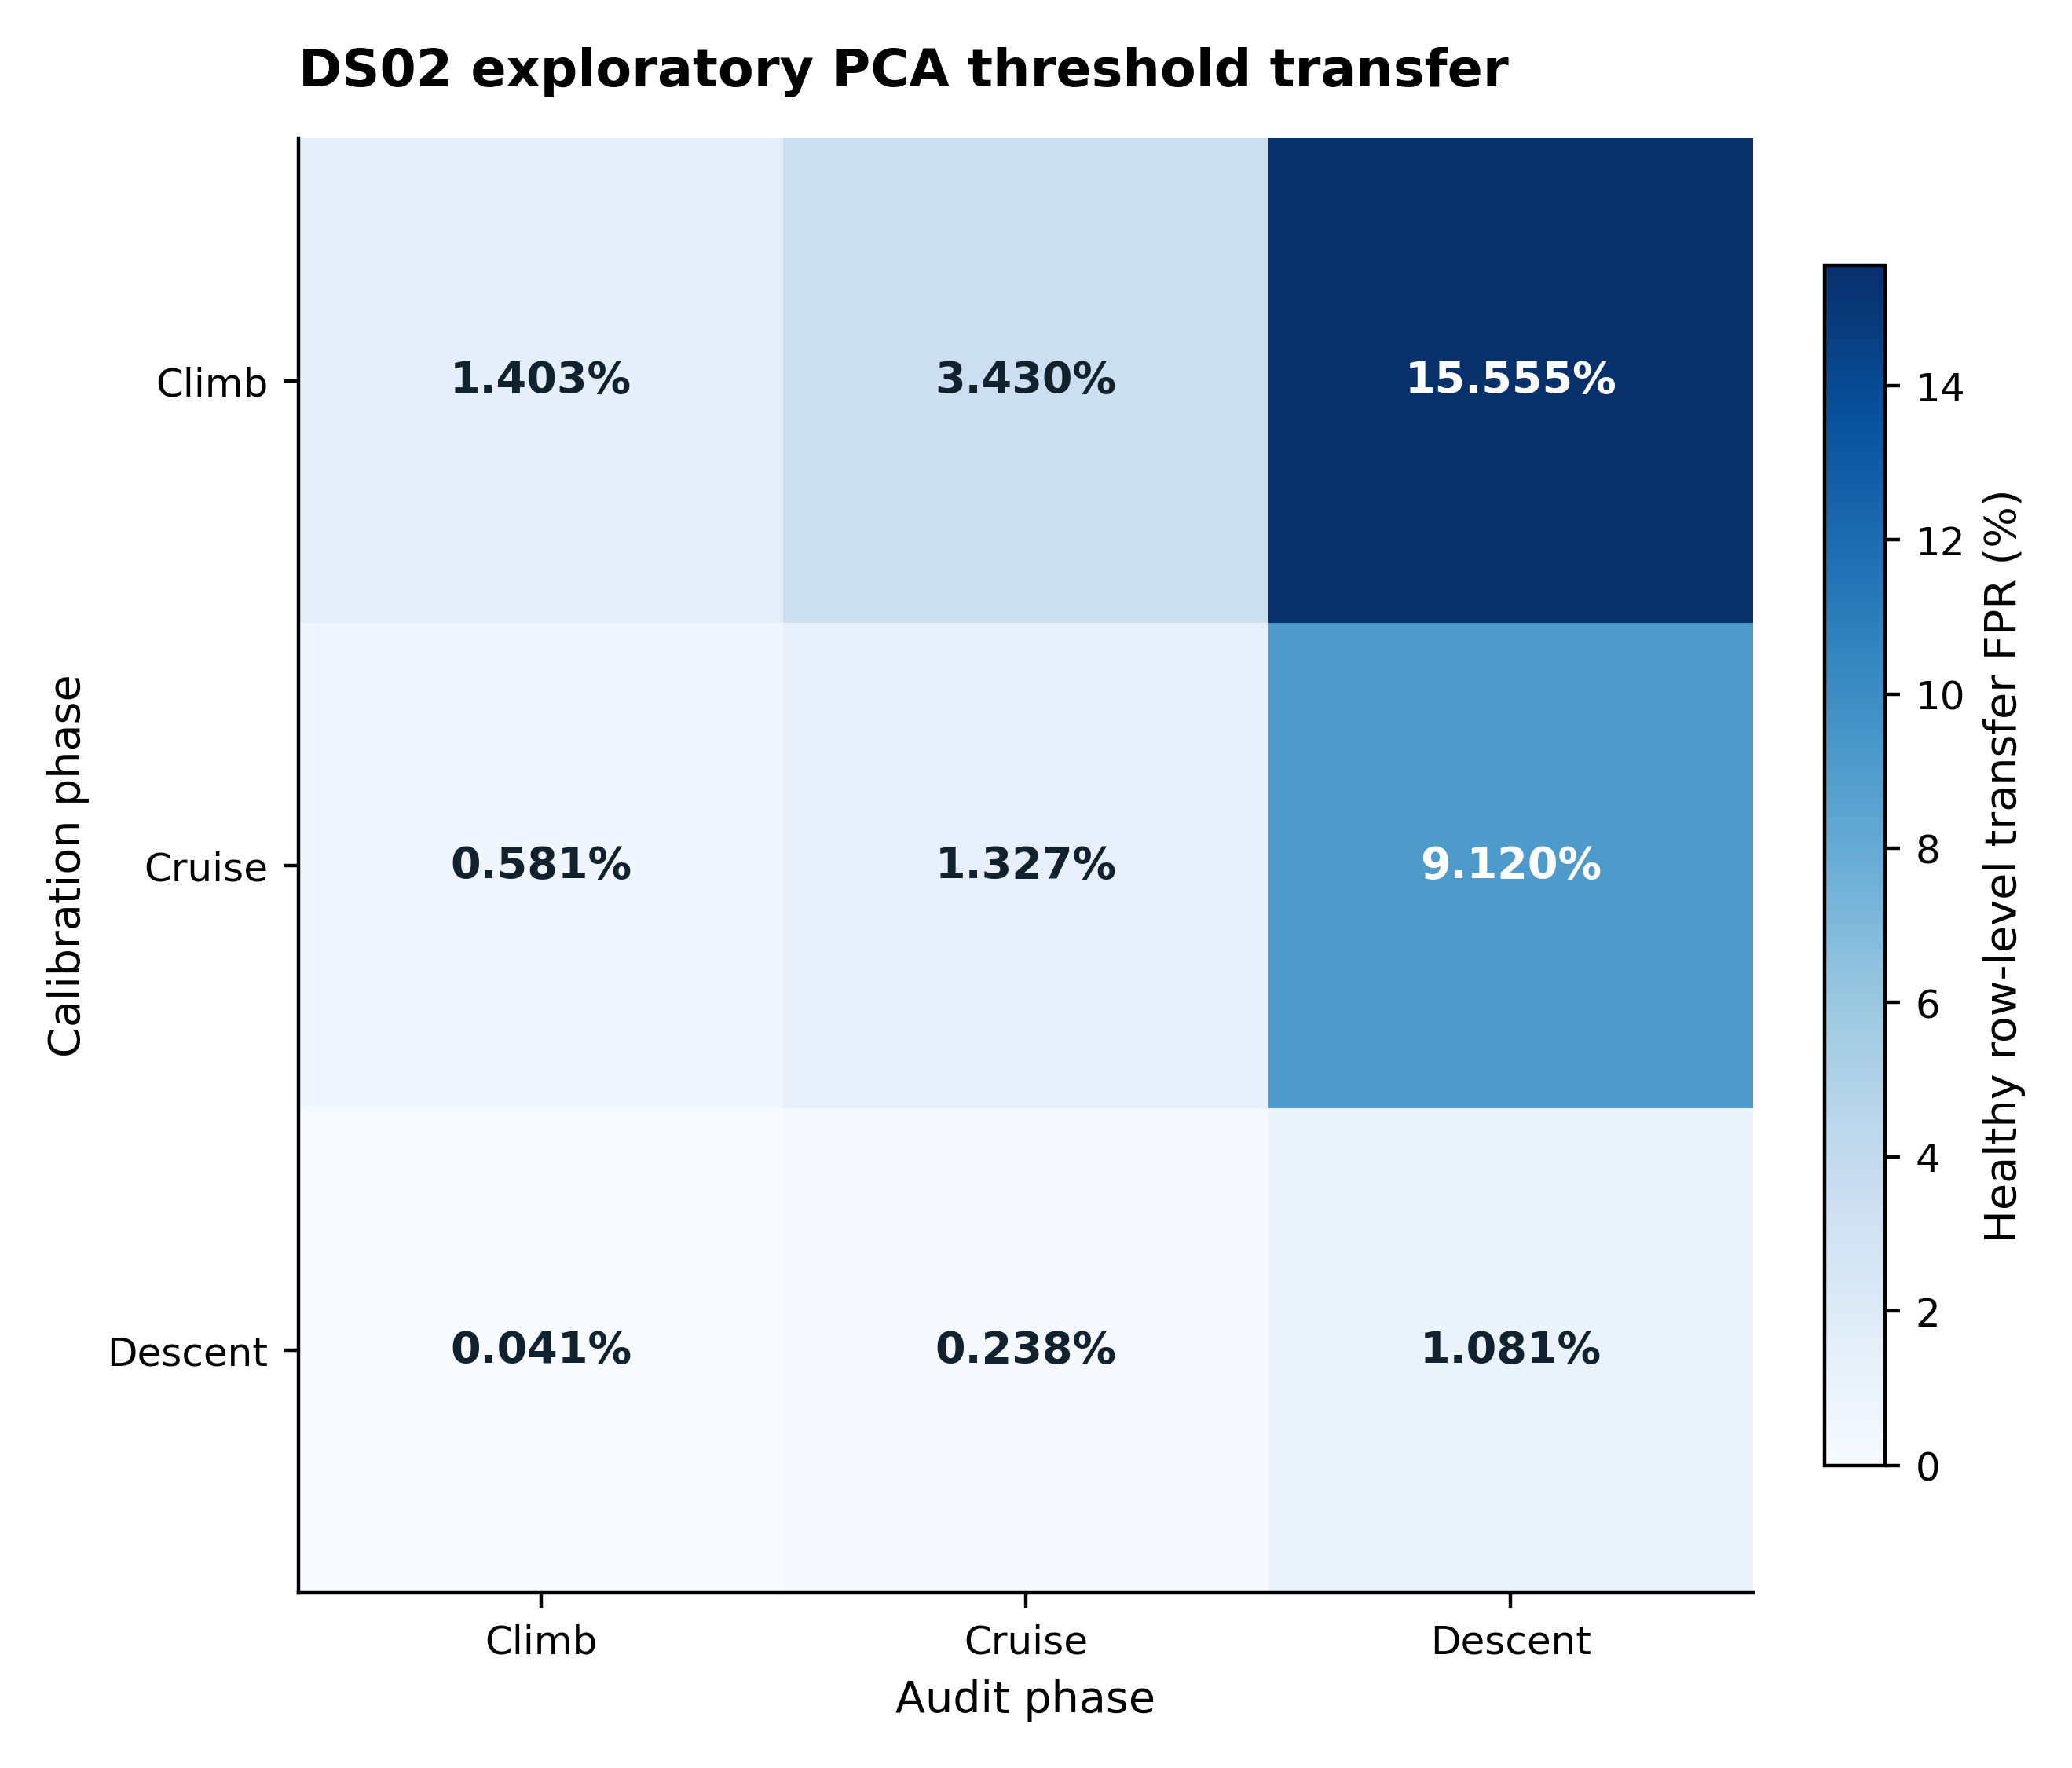
\includegraphics[width=0.94\textwidth]{figures/figure_3_cross_phase_transfer.png}
\caption{DS02 exploratory PCA cross-phase threshold transfer at the nominal 1\% target. Calibration phase is shown vertically and healthy audit phase horizontally. Each cell is the held-out transfer FPR after phase-specific calibration, not pooled phase FPR. Diagonal cells are same-phase audit FPRs and are not constrained to exactly 1\%.}
\end{figure*}

\subsection{Interpretation of the Main Finding}\label{interpretation-of-the-main-finding}

The central observation is a calibration-stability failure, not simply a higher descent FPR. At the primary pooled healthy calibration target, the phase-wise healthy row-level FPRs differed on DS02 and DS03 across the three tested implementations. An overall \(P(\mathrm{alarm}\mid\mathrm{healthy})\) is an exposure-weighted average and can therefore conceal differences in \(P(\mathrm{alarm}\mid\mathrm{healthy},\mathrm{phase})\). The nominal target specifies a calibration quantile; it does not guarantee the same healthy alarm probability in each audit phase.

Cross-phase transfer provides a distinct check: a threshold estimated from healthy scores in one phase need not preserve its nominal operating characteristic in another. The observed worst off-diagonal FPRs, including climb-calibrated thresholds applied to descent, demonstrate nonuniform transfer in these N-CMAPSS audits. They are maxima over transfer cells, not pooled-threshold phase FPRs or projected deployment rates. Neither the conditional differences nor the transfer results identify a causal mechanism.

\subsection{Sensitivity to Operating-Condition Correction}\label{sensitivity-to-operating-condition-correction-1}

In DS02 exploratory PCA analysis, static, derivative-based, and finite-history corrections did not eliminate the phase-dependent FPR pattern. Cross-detector consistency was evaluated under the selected finite-history correction. In that PCA comparison, descent-minus-climb and descent-minus-cruise FPR contrasts remained positive under static, static-plus-derivative, and finite-history operating-condition correction. Thus, the tested specifications were insufficient to make healthy row-level FPR phase-stable at the evaluated pooled threshold. This is a bounded statement about these fitted corrections on DS02; the three-way correction comparison was not repeated as a frozen DS03 endpoint. Whether correction-scheme sensitivity is similarly weak for Isolation Forest and LSTM was not tested and remains an open robustness question.

Finite sensor response, omitted operating variables, longer state history, path dependence, phase-transition effects, and model misspecification are possible explanations for residual score variation. They are hypotheses rather than findings: the present contrasts do not separate these possibilities causally, exclude other dynamic effects, or establish any particular physical mechanism.

\subsection{Implications for Anomaly-Detector Evaluation}\label{implications-for-anomaly-detector-evaluation}
\begin{figure*}[t]
\centering
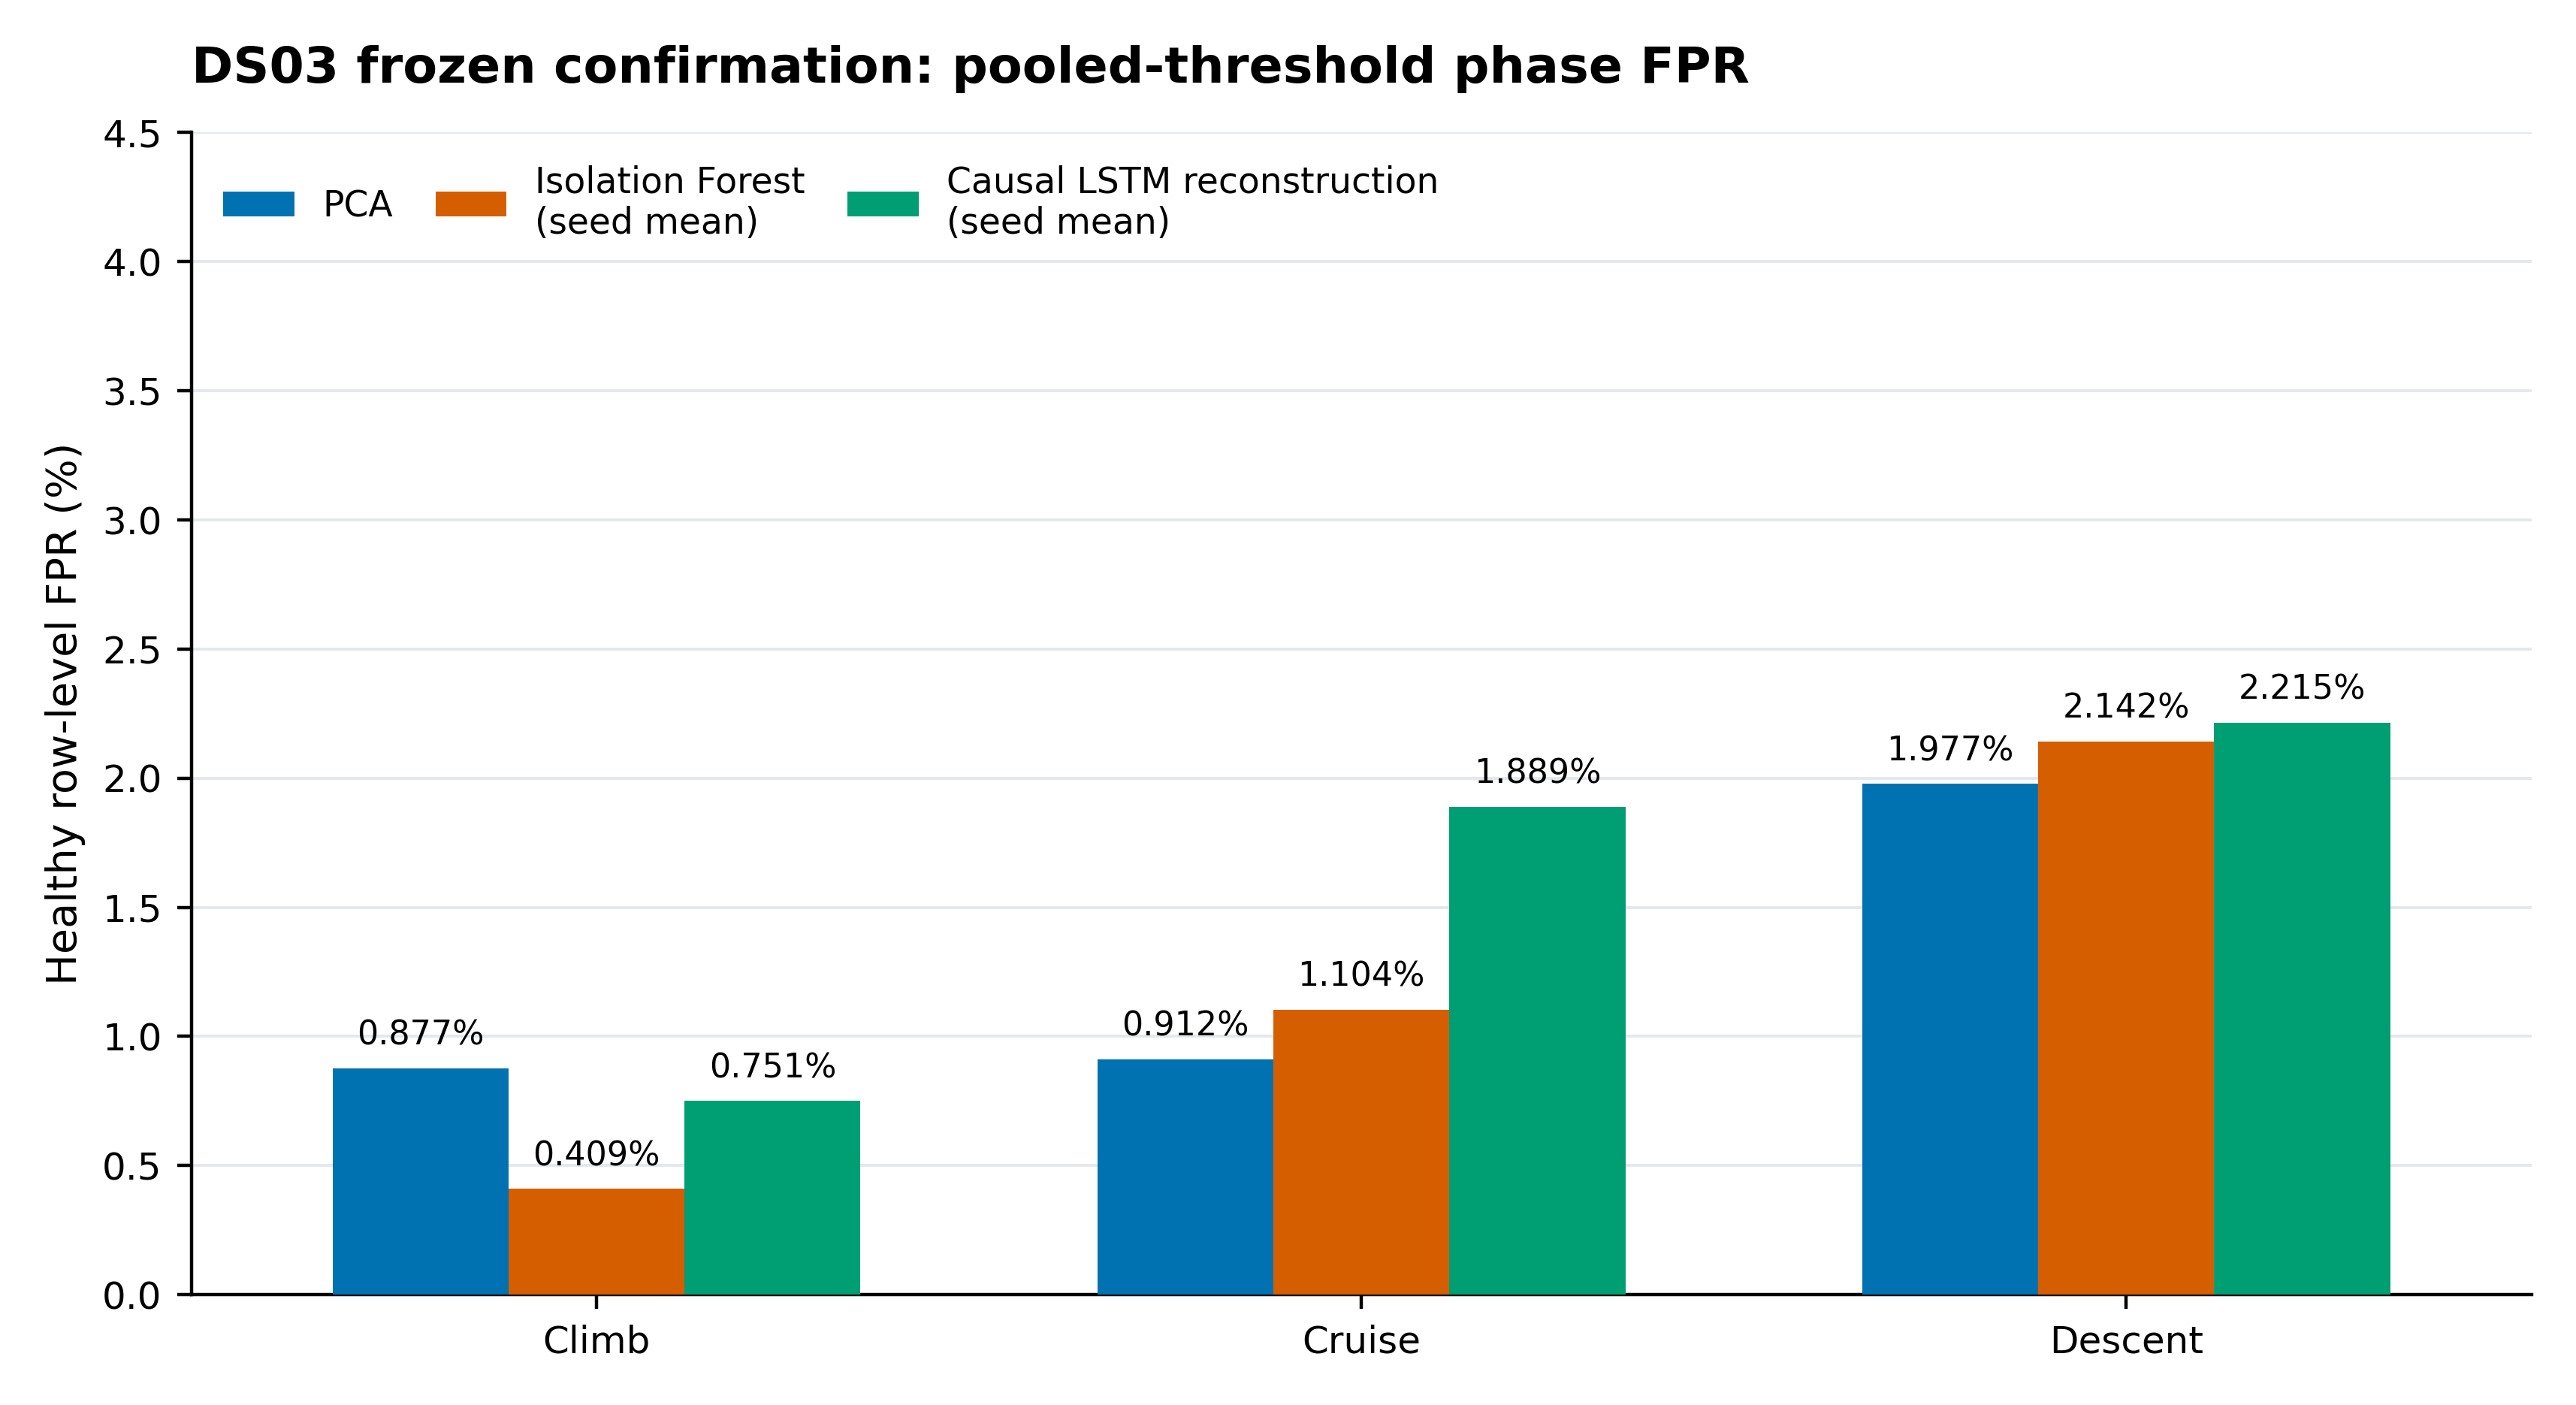
\includegraphics[width=0.94\textwidth]{figures/figure_4_ds03_phase_fpr.png}
\caption{DS03 frozen confirmatory healthy row-level FPR at the nominal 1\% pooled calibration target. PCA is a single run; Isolation Forest and the causal LSTM sequence-reconstruction network are arithmetic three-seed means. Bars show pooled-threshold phase FPR, not cross-phase transfer FPR. The vertical scale matches Fig. 2; no seed-mean confidence interval was executed.}
\end{figure*}

Overall FPR, AUROC, PR-AUC, and F1 remain useful summaries for their respective questions, but none alone describes the healthy false-alarm behavior of a selected threshold in each operating context. Under nonstationary full-flight operation, phase-wise FPR, conditional calibration, and cross-phase threshold transfer expose behavior that an aggregate score or rate can hide. Engine-level contrasts and engine-then-flight uncertainty summaries further distinguish a pooled direction from heterogeneous individual-engine outcomes. The three DS02 and six DS03 official-test engines make individual-engine reversals material to the interpretation.

In practice, report phase-conditional healthy FPR alongside pooled FPR, audit threshold transfer across normal operating contexts, and inspect engine-level heterogeneity. Consider context-specific calibration only after checking that it does not degrade fault sensitivity. Any context-aware calibration would require validation on independently sourced or real full-flight data before operational interpretation. These are evaluation steps, not evidence that an alternative threshold policy is superior.

\subsection{Discovery--Confirmation Design}\label{discoveryconfirmation-design}

DS02 allowed exploratory correction challenges and cross-detector checks before the analysis choices were frozen. The subsequent one-shot evaluation on the DS03 independent confirmatory subset met the pre-specified pooled directional point-estimate rule: both descent contrasts were positive for PCA and for the seed means of Isolation Forest and LSTM. This reproduces the pooled directional pattern under the frozen rule; it does not establish uniform replication for every engine or seed.

Qualifications remain material. Three of 42 DS03 per-engine detector/seed rows were directional exceptions, all associated with LSTM seed 2, and each individual LSTM descent-minus-cruise hierarchical-bootstrap interval included zero. Separately, the DS02 LSTM seed-0 selection reached the pre-specified 600-epoch ceiling while validation loss was still improving; it should not be described as converged. Reporting these exceptions and the training limitation narrows the inference but makes the confirmation claim auditable.

\subsection{Limitations and Scope}\label{limitations-and-scope}

N-CMAPSS is a simulation driven by recorded flight conditions; these results do not establish validity on real aircraft. Phase labels require complete-flight trajectories and serve retrospective stratification, not online phase detection. Oracle health-state labels select healthy rows for fitting, calibration, and retrospective FPR evaluation; they are never numerical detector inputs. The analysis does not estimate fault recall, detection delay, or overall anomaly-detection superiority.

Phase-rule sensitivity was explored on DS02 with an alternative altitude-rate definition, but the frozen DS03 confirmation used only the primary retrospective 90\%-altitude rule. The engine sets are limited. Hierarchical-bootstrap intervals resample engines and flights and are best read as uncertainty summaries for the observed N-CMAPSS sets, not precise population estimates. Stochastic-detector seed means are descriptive point summaries rather than inferential estimates: the retained outputs do not provide a valid interval for the fixed three-seed arithmetic mean, and averaging individual-seed interval endpoints would not supply one. All three individual-seed DS03 LSTM descent-minus-cruise intervals include zero. All three tested detector implementations share preprocessing, correction, and calibration structure, so their agreement does not establish detector independence. The static, derivative-based, and finite-history corrections tested on DS02 are not exhaustive.

The present study establishes an empirical calibration-stability concern rather than a causal explanation. Mechanism identification, broader robustness to alternative phase definitions, correction-scheme sensitivity across additional detector families, and independent reimplementation remain separate validation targets.

Before treating an anomaly score as a condition-invariant health indicator, a monitoring study should audit whether healthy calibration remains stable across its normal operating contexts.

\section{Conclusion}\label{conclusion}

This study asked whether nominal pooled healthy FPR calibration remains stable across normal flight phases during full-flight aero-engine operation. In the exploratory N-CMAPSS DS02 analysis, healthy phase-wise FPR differed across climb, cruise, and descent for PCA, Isolation Forest, and the causal LSTM sequence-reconstruction network. In the exploratory DS02 PCA comparison, the tested static, derivative-based, and finite-history operating-condition correction schemes did not eliminate the observed dependence. Under the frozen one-shot DS03 protocol, the pre-specified pooled directional pattern was reproduced on the independent confirmatory subset.

Aggregate healthy FPR can therefore conceal operating-context-dependent alarm behaviour, and calibration stability across normal conditions warrants explicit auditing. The evidence remains limited to simulated N-CMAPSS data, retrospective phase labels, and small engine sets. It does not assess fault recall or detection delay, establish independence among the tested implementations, or identify a causal mechanism. Future work should test the calibration-audit question on real or independently sourced full-flight data and evaluate whether context-aware calibration can reduce phase dependence without compromising fault sensitivity.
\begin{thebibliography}{12}
\bibitem{ref1} M. Arias Chao, C. Kulkarni, K. Goebel, and O. Fink, ``Aircraft Engine Run-to-Failure Dataset under Real Flight Conditions for Prognostics and Diagnostics,'' \emph{Data}, vol.~6, no. 1, art. 5, 2021. doi: \href{https://doi.org/10.3390/data6010005}{10.3390/data6010005}.
\bibitem{ref2} S. Borguet and O. Léonard, ``Assessment of an Anomaly Detector for Jet Engine Health Monitoring,'' \emph{International Journal of Rotating Machinery}, 2011. doi: \href{https://doi.org/10.1155/2011/942576}{10.1155/2011/942576}.
\bibitem{ref3} D. Dimogianopoulos, J. D. Hios, and S. D. Fassois, ``Aircraft Engine Health Management via Stochastic Modelling of Flight Data Interrelations,'' \emph{Aerospace Science and Technology}, vol.~16, no. 1, pp.~70--81, 2012. doi: \href{https://doi.org/10.1016/j.ast.2011.03.002}{10.1016/j.ast.2011.03.002}.
\bibitem{ref4} H. Noura and J. Wiig, ``Flight Stage Normalization of HUMS Indicators,'' Vertical Flight Society Forum 62, 2006. doi: \href{https://doi.org/10.4050/VFS-F62-051}{10.4050/VFS-F62-051}.
\bibitem{ref5} V. Zaccaria, A. D. Fentaye, M. Stenfelt, and K. G. Kyprianidis, ``Probabilistic Model for Aero-Engines Fleet Condition Monitoring,'' \emph{Aerospace}, vol.~7, no. 6, art. 66, 2020. doi: \href{https://doi.org/10.3390/aerospace7060066}{10.3390/aerospace7060066}.
\bibitem{ref6} W. Zhao, Y. Guo, and H. Sun, ``Research on an Adaptive Threshold Setting Method for Aero-Engine Fault Detection Based on KDE-EWMA,'' \emph{Journal of Aerospace Engineering}, vol.~35, no. 6, 2022. doi: \href{https://doi.org/10.1061/(ASCE)AS.1943-5525.0001483}{10.1061/(ASCE)AS.1943-5525.0001483}.
\bibitem{ref7} M. Ulmer, J. Zgraggen, and L. Goren Huber, ``A Generic Machine Learning Framework for Fully-Unsupervised Anomaly Detection with Contaminated Data,'' \emph{International Journal of Prognostics and Health Management}, vol.~15, no. 1, 2024. doi: \href{https://doi.org/10.36001/IJPHM.2024.v15i1.3589}{10.36001/IJPHM.2024.v15i1.3589}.
\bibitem{ref8} C. Ramírez \emph{et al.}, ``Fault Detection and Monitoring Using a Data-Driven Information-Based Strategy: Method, Theory, and Application,'' \emph{Mechanical Systems and Signal Processing}, vol.~228, art. 112403, 2025. doi: \href{https://doi.org/10.1016/j.ymssp.2025.112403}{10.1016/j.ymssp.2025.112403}.
\bibitem{ref9} S. Yan, Y. Zhang, and X. Gong, ``A Physics-Guided Spatio-Temporal Attention Graph Network for Unsupervised Aircraft Engine Anomaly Detection,'' \emph{Mathematics}, vol.~14, no. 18, art. 3413, 2026. doi: \href{https://doi.org/10.3390/math14183413}{10.3390/math14183413}.
\bibitem{ref10} P. Cheng and Q. Miao, ``CruiseBench: A Real-Flight-Aligned N-CMAPSS Benchmark for Engine RUL Prediction,'' 2026, preprint. arXiv: \href{https://arxiv.org/abs/2607.19380}{2607.19380}.
\bibitem{ref11} J.-R. Massé, A. Humeau, P. Lalonde, and A. Alimardani, ``Placement of Alert Thresholds on Abnormality Scores,'' \emph{PHM Society European Conference}, vol.~2, no. 1, 2014. doi: \href{https://doi.org/10.36001/phme.2014.v2i1.1542}{10.36001/phme.2014.v2i1.1542}.
\bibitem{ref12} J. D. Papastavrou and M. R. Lehto, ``Improving the Effectiveness of Warnings by Increasing the Appropriateness of Their Information Content: Some Hypotheses About Human Compliance,'' \emph{Safety Science}, vol.~21, no. 3, pp.~175--189, 1996. doi: \href{https://doi.org/10.1016/0925-7535(95)00060-7}{10.1016/0925-7535(95)00060-7}.
\end{thebibliography}




\begin{table*}[t]
\centering
\footnotesize
\caption{Dataset and frozen protocol summary. DS02 is exploratory discovery; DS03 is an independent confirmatory N-CMAPSS subset under the frozen one-shot protocol. This design table contains no pooled phase-FPR or cross-phase transfer-FPR outcomes; seed means are not applicable.}
\begin{tabular}{p{0.20\textwidth}p{0.36\textwidth}p{0.36\textwidth}}
\hline
Item & DS02 discovery (exploratory) & DS03 independent confirmatory subset \\
\hline
Role & Discovery, correction sensitivity, detector development & Frozen one-shot confirmation \\
Model-fitting engines & 2, 5, 10, 16 & 1, 2, 3, 5, 6, 7, 9 \\
LSTM epoch-selection fitting engines & 2, 5, 10 & 1, 2, 3, 5, 6, 7 \\
LSTM epoch-selection validation engine & 16 & 9 \\
Threshold-calibration engines & 18, 20 & 4, 8 \\
Official audit/test engines & 11, 14, 15 & 10, 11, 12, 13, 14, 15 \\
Phase-label role & Retrospective full-flight stratification; cruise spans the first through last sample at or above the minimum plus 90\% of each flight's observed altitude range & Same frozen retrospective primary rule \\
Nominal pooled healthy row-FPR targets & 0.5\%, 1\%, 2\%; 1\% primary & Same frozen targets and primary target \\
Detector implementations & PCA; Isolation Forest; causal LSTM sequence reconstruction & Same frozen implementations \\
Operating-condition correction & Static, static + derivative, and finite-history compared for PCA exploratorily; finite-history used for canonical detector results & Finite-history only; no DS03 correction-variant selection \\
\hline
\end{tabular}
\par\vspace{3pt}\footnotesize Health-state annotations select healthy rows for retrospective fitting, calibration, and FPR evaluation; they are not detector features. Phase labels are retrospective strata, not an online phase detector.
\end{table*}
\begin{table*}[t]
\centering
\footnotesize
\caption{DS02 exploratory canonical results at the nominal 1\% pooled healthy calibration target. Phase FPR columns use the pooled threshold; the final column is the worst off-diagonal cross-phase \textbf{transfer} FPR and is not a pooled phase FPR. Isolation Forest and LSTM rows are arithmetic means across the tested seeds, with no seed-mean confidence interval.}
\resizebox{\textwidth}{!}{\begin{tabular}{lrrrrrrr}
\hline
Detector & Overall FPR (\%) & Climb FPR (\%) & Cruise FPR (\%) & Descent FPR (\%) & Descent − climb (pp) & Descent − cruise (pp) & Worst cross-phase transfer FPR (\%) \\
\hline
PCA & 1.363\% & 0.125\% & 0.428\% & 3.459\% & +3.335 pp & +3.031 pp & 15.555\% \\
Isolation Forest (seed mean) & 1.127\% & 0.268\% & 0.558\% & 2.487\% & +2.219 pp & +1.928 pp & 27.281\% \\
Causal LSTM reconstruction (seed mean) & 1.118\% & 0.488\% & 0.729\% & 2.080\% & +1.592 pp & +1.351 pp & 5.954\% \\
\hline
\end{tabular}}
\end{table*}
\begin{table*}[t]
\centering
\footnotesize
\caption{Frozen DS03 confirmatory pooled results at the nominal 1\% pooled healthy calibration target. Climb/cruise/descent columns are pooled-threshold phase FPRs, not cross-phase transfer FPRs. Isolation Forest and LSTM point estimates are arithmetic seed means; the 95\% hierarchical-bootstrap contrast intervals apply only to individual detector runs, so no interval is assigned to a seed mean.}
\resizebox{\textwidth}{!}{\begin{tabular}{lrrrrrrr}
\hline
Detector & Climb FPR (\%) & Cruise FPR (\%) & Descent FPR (\%) & Descent − climb (pp) & Run-level 95\% CI (pp) & Descent − cruise (pp) & Run-level 95\% CI (pp) \\
\hline
PCA & 0.877\% & 0.912\% & 1.977\% & +1.100 pp & {[}+0.434 pp, +1.785 pp{]} & +1.066 pp & {[}+0.560 pp, +1.573 pp{]} \\
Isolation Forest (seed mean) & 0.409\% & 1.104\% & 2.142\% & +1.733 pp & --- & +1.038 pp & --- \\
Causal LSTM reconstruction (seed mean) & 0.751\% & 1.889\% & 2.215\% & +1.464 pp & --- & +0.325 pp & --- \\
\hline
\end{tabular}}
\par\vspace{3pt}\footnotesize \emph{Note:} 3 of 42 per-engine detector/seed directional rows were exceptions, all associated with LSTM seed 2. All three individual LSTM descent-minus-cruise bootstrap intervals include zero. No confidence interval is reported for arithmetic seed means because no seed-mean bootstrap interval was executed. Individual-seed interval tables belong in the supplement; cross-phase transfer FPR is not tabulated here.
\end{table*}
\end{document}
